\documentclass[12pt]{article}
\usepackage[utf8]{inputenc}
\usepackage{amsmath}
\usepackage[T1]{fontenc}

\title{ECE 3413 Lab 08\\*DC Motor Model for Open-loop Control in MATLAB Simulink}
\author{Leomar Dur\'an}
\date{${12}^{\text{th}}$ April 2023}

\usepackage[natbib,style=apa6]{biblatex}
\addbibresource{main.bib}
\defbibheading{bibliography}[\refname]{%
  \section*{\centering #1}%
}%

\usepackage{hyperref}

\usepackage{cancel}
\usepackage[per-mode=symbol]{siunitx}
\newcommand*\siexpr[2][]{\SI[parse-numbers=false,#1]{#2}}%
\usepackage{xfrac}
\usepackage{amssymb}
\newcommand*\transpose{\mathsf{T}}

\usepackage{mathtools}%
\DeclarePairedDelimiter\brao()%
\DeclarePairedDelimiter\brac[]%
\DeclarePairedDelimiter\braco[)%
\DeclarePairedDelimiter\braoo][%
\DeclarePairedDelimiter\Brac\{\}%
\DeclarePairedDelimiter\abs||
\DeclarePairedDelimiter\norm\lVert\rVert%
\DeclarePairedDelimiter\piecefn\{.
\DeclarePairedDelimiter\evalat.|

\usepackage{lib/nonfloatenvirons}
\usepackage{booktabs}
\newcommand\ra[1]{\renewcommand*\arraystretch{#1}}
\ra{1.25}

\usepackage{minted}
\newcommand\matlab{matlab}

\usepackage{adjustbox}
\newcommand{\setprime}[2][1]{%
    {#2}^{%
        \raisebox{1pt}{%
            \scalebox{0.5}{%
                \itshape\sffamily\uppercase%
                \expandafter{%
                    \romannumeral#1%
                }%
            }%
        }
    }%
}%
\newcommand*\mcadj[7]%
% {#columns}{col spec}{rotation}{adjust spec}
% {before rotated text}{rotated text}{after rotated text}
{%
    \multicolumn{#1}{#2}{%
        \rlap{%
            #5\adjustbox{rotate=#3,#4}{#6}~#7%
        }%
    }%
}

\usepackage{pdfpages}
\usepackage{standalone}
\usepackage{matlab}

\usepackage[skip=\baselineskip,indent=0pt]{parskip}
\setlength\parindent{0pt}

\usepackage[shortlabels]{enumitem}

\def\hr{{\par\noindent\rule{\textwidth}{0.4pt}}}

\begin{document}

\maketitle
\newpage

\section{Introduction}

In this experiment, we build the DC motor using a series negative feedback close-loop system,
testing both the angular velocity and position to ensure that the motor works as expected.

We will also experiment with the gains, moment of inertia, and the mechanical system's damping ratio as parameters of the DC motor's simulation.

\section{Procedure}\label{sec:procedure}

\subsection{Task 0 -- Modeling the DC Motor}\label{ssc:dc motor model}

In this lab, we simulate a DC motor according to the system on page~\pageref{pdf:dc motor model}.
The parameters for this are in the script in \nameref{app} subsection~\ref{sap:default params}.

The motor uses integration in the Laplace domain.
Thus, the integrator system used is merely as shown on page~\pageref{pdf:integrators}.

The DC motor is placed in a simple IPO system
on page~\pageref{pdf:dc motor system}
as the professor to analyze the motor.
Additionally, we have added a second integrator and a modulus channel to wrap the output around $\braco{0, 2\pi}$.
This produces the angular position (or angle in radians).

The motor can be mathematically described using the model
\begin{equation}
    \brac*{
        \begin{matrix}
            J\ddot\theta\brao*t \\* L\dot{I}\brao*t
        \end{matrix}
    } =
    \brac*{
        \begin{matrix}
            K_t & 0 & -b \\*
            -R & 1 & -K_e \\*
        \end{matrix}
    }\brac*{
        \begin{matrix}
            I \\* V \\* \dot\theta\brao*t
        \end{matrix}
    }.
\end{equation}

\includepdf[pages=2,landscape=true,pagecommand=\label{pdf:dc motor model}]{drawings/lab08_openloop_control_slx.pdf}
\includepdf[pages=3,landscape=true,pagecommand=\label{pdf:integrators}]{drawings/lab08_openloop_control_slx.pdf}
\includepdf[pages=1,landscape=true,pagecommand=\label{pdf:dc motor system}]{drawings/lab08_openloop_control_slx.pdf}

\subsection{Task 1 -- Varying the gains}

We plotted the result of modeling the DC motor with the gains given in \eqref{eq:gains}, representing both the armature torque constant and the back EMF from the motor.

\begin{equation}\label{eq:gains}
    K \in \Brac*{\begin{matrix}.01, & .02, & .3, & .4, & 1, & 2\end{matrix}}.
\end{equation}

We automated this process by using the script in \nameref{app} subsection~\ref{sap:vary gains}.

\subsection{Task 2 -- Plotting the angular velocity response}

After this, we see the effect of the default parameters on the motor, using the script in \nameref{app} subsection~\ref{sap:plotting angular velocity}.

\subsection{Tasks 03(a), 4 -- Varying the moment of inertia of the motor}

We plotted the result of modeling the DC motor with the moments of inertia given in \eqref{eq:moments of inertia}.

\begin{equation}\label{eq:moments of inertia}
    J \in \Brac*{\begin{matrix}.1, & 1, & 5\end{matrix}}.
\end{equation}

We automated this process by using the script in \nameref{app} subsection~\ref{sap:vary moment of inertia}.

\subsection{Tasks 03(b), 4 -- Varying the damping ratio of the mechanical system}

We plotted the result of modeling the DC motor with the damping ratios of the mechanical systems in \eqref{eq:damping ratios}.

\begin{equation}\label{eq:damping ratios}
    b \in \Brac*{\begin{matrix}.01, & .1, & .2\end{matrix}}.
\end{equation}

We automated this process by using the script in \nameref{app} subsection~\ref{sap:vary damping ratio}.


\subsection{Task 05 -- Parameters to repeat the angle period}

Finally, we use the scope for the angular position mentioned in subsection~\ref{ssc:dc motor model}.

The parameters for this are in the script in \nameref{app} subsection~\ref{sap:repeat angle params}. 
Rather than the default time of $\SI{10.0}\second$,
we use $\SI{100.0}\second$
to show the angle period repeating.

\section{Results}

\subsection{Task 1 -- Varying the gains}

\begin{figure}
    \centering
    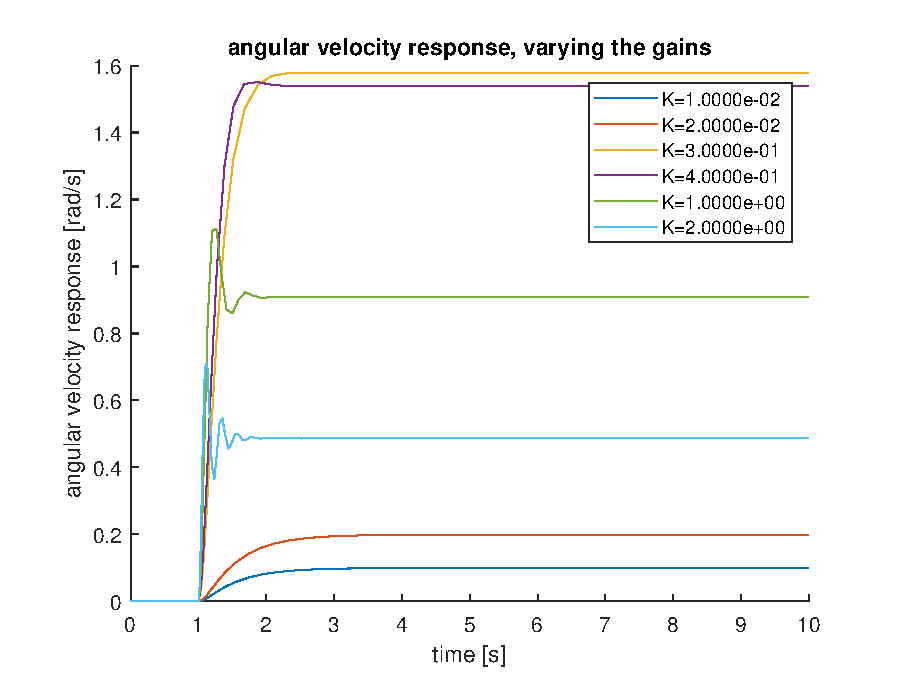
\includegraphics[width=\linewidth]{img/task01_varying_gains.eps}
    \caption{Effect of gains on the angular velocity response.}
    \label{fig:gains on angular velocity}
\end{figure}

Here we can see that while $K < .3$, the angular velocity's response seems to to be approaching critically damped from overdamped.
The gains make the final value increase.
In the interval $K \in \braoo{.3, .4}$, we see the final value being to decrease and now the angular velocity becomes underdamped. We see the overshoot and the settling time begin to increase with $K$.

\subsection{Task 2 -- Plotting the angular velocity response}

\begin{figure}
    \centering
    \includegraphics[width=\linewidth]{img/task02_plot_angular_velocity.eps}
    \caption{Plot of the angular velocity response.}
    \label{fig:plot of angular velocity}
\end{figure}

This is the angular velocity using the default parameters for the DC motor model.

\subsection{Tasks 03(a), 4 -- Varying the moment of inertia of the motor}\label{moment of inertia, task}

\begin{figure}
    \centering
    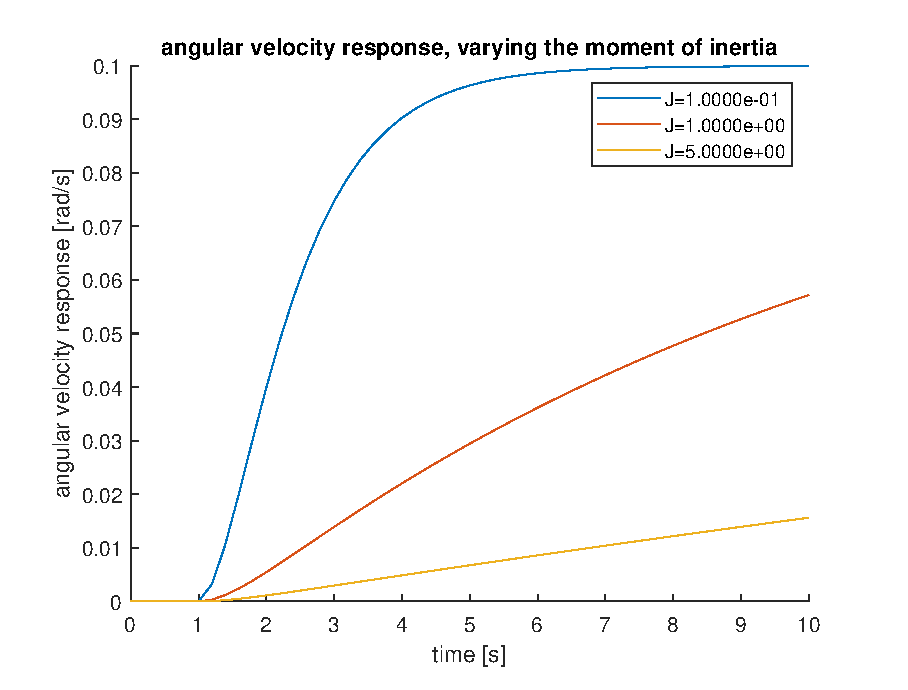
\includegraphics[width=\linewidth]{img/task03a_varying_moment_of_inertia.eps}
    \caption{Effect of the moment of inertia on the angular velocity response.}
    \label{fig:moment of inertia on angular velocity}
\end{figure}

\subsection{Tasks 03(b), 4 -- Varying the damping ratio of the mechanical system}\label{mechanical sys damping ratio, task}

\begin{figure}
    \centering
    \includegraphics[width=\linewidth]{img/task03b_varying_mechanical_sys_damping_ratio.eps}
    \caption{Effect of the damping ratio of the mechanical system on the angular velocity response.}
    \label{fig:mechanical system damping ratio on angular velocity}
\end{figure}

\subsection{Task 05 -- The angular position vs time}

\begin{figure}
    \centering
    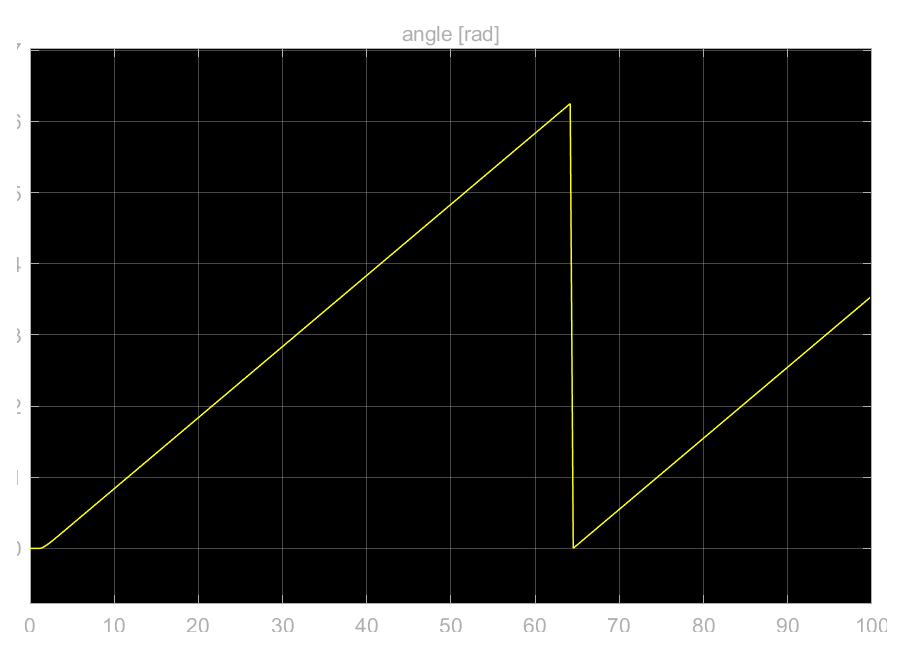
\includegraphics[width=\linewidth]{img/task05_angular_position.eps}
    \caption{The angular position of the motor.}
    \label{fig:angular position of motor}
\end{figure}

This is what we expect of the DC motor. We see the angle rising linearly and completing a rotating at $\theta\brao*t = 2\pi$ while it continues to rise linearly. This tarts as soon as $t = \SI1\second$.

\section{Discussion}
In this lab, we learned how to model a DC motor with a series closed-loop negative feedback system. We saw that the model behaved as expected rotating linearly and analyzed the effects of gain on the dampness of the function.

Additionally, let's consider the 
moment of inertia of the motor
and the damping ratio of the mechanical system.

In Fig.~\ref{fig:moment of inertia on angular velocity}, we see that increasing the moment of inertia decreases the value of the final value of the response while making the system become less stable (forming a ramp). Opposite this, decreasing the moment of inertia makes the final value much larger while increasing the dampness of the system. The value at $J = .1$ appears to be overdamped.

In Fig.~\ref{fig:mechanical system damping ratio on angular velocity}, the damping ratio of the mechanical system seems to have a similar affect, being inversely proportional to the final value, but without affecting the system's stability.

Additionally, the increase of the final value is more dramatic as the damping ratio decreases, compared to the decrease in final value being more dramatic as the moment of inertia increases.

\newpage
\printbibliography

\newpage
\appendix
\section{Appendix}\label{app}

\subsection{Task 00 -- Default parameters, Matlab script}\label{sap:default params}
\inputminted{matlab}{src/lab08_task00_default_dc_motor_motor_params.m}

\hr{}

\subsection{Task 01 -- Varying the gains, Matlab script}\label{sap:vary gains}
\inputminted{matlab}{src/lab08_task01_vary_gain.m}

\hr{}

\subsection{Task 02 -- Plotting the angular velocity response, Matlab script}\label{sap:plotting angular velocity}
\inputminted{matlab}{src/lab08_task02_plot_angular_velocity.m}

\hr{}

\subsection{Task 03(a) -- Varying the moment of inertia of the motor, Matlab script}\label{sap:vary moment of inertia}
\inputminted{matlab}{src/lab08_task03a_vary_motor_moment_of_inertia.m}

\subsection{Task 03(b) -- Varying the damping ratio of the mechanical system, Matlab script}\label{sap:vary damping ratio}
\inputminted{matlab}{src/lab08_task03b_vary_mechanical_sys_damping.m}

\subsection{Task 05 -- Parameters to repeat the angle period, Matlab script}\label{sap:repeat angle params}
\inputminted{matlab}{src/lab08_task05_angle_repeat_params.m}

\end{document}
